\section{Instrumentação}
\paragraph{}Nesta sessão todos os instrumentos utilizados para o desenvolvimento do projeto serão descritos e a metodologia dos testes que foram realizados.

\subsection{Eletroestimulador}
\paragraph{}O eletroestimulador foi desenvolvido no Laboratório de Instrumentação Biomédica (LIB) como projeto de final de curso do aluno Anderson Francisco da Costa Souza\cite{Anderson34}, ele é constituído basicamente de um microcontrolador ALGUMACOISA que realiza a comunicação com o computador, além de providenciar o pulso de estimulação. Este pulso depois passa por diversos circuitos até passar em um estágio de saída em par Darlington para injetar a corrente no músculo.

\subsubsection{Pulso de Estimulação}

\begin{figure}[H]
	\centering
	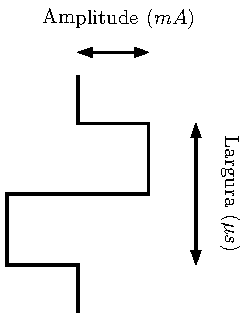
\includegraphics[width=0.5\textwidth,angle=90]{pulso_estimulacao.pdf}
	\caption{Pulso de estimulação utilizado, podendo-se variar tanto amplitude quanto largura do pulso.}
	\label{fig:pulso_estimulacao}
\end{figure}

\paragraph{}O pulso de estimulação possui formato bifásico, e é possível modificar amplitude, largura e frequência através de \textit{software}.

\subsubsection{Eletrodos de Contato}
Os eletrodos de contato utilizados foram eletrodos quadrados, autoadesivos de $5 x 5 cm$.

\subsection{Goniômetro}

\begin{figure}[H]
	\centering
	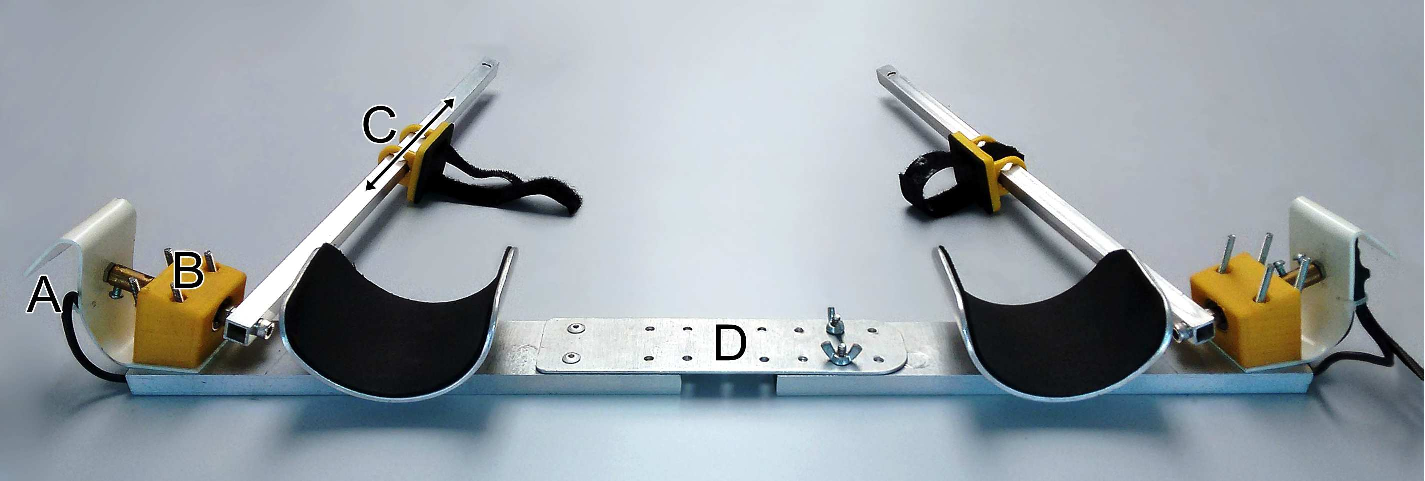
\includegraphics[width=0.8\textwidth]{aparatops.pdf}
	\caption{Goniômetro desenvolvido pelo LIB. (A) e (B) formam um conjunto de sensores, (C) é um prendedor regulável, e (D) é um regulador da largura do goniômetro.}
	\label{fig:aparatops}
\end{figure}

\subsection{Interface com o Usuário}

\begin{figure}[H]
	\centering
	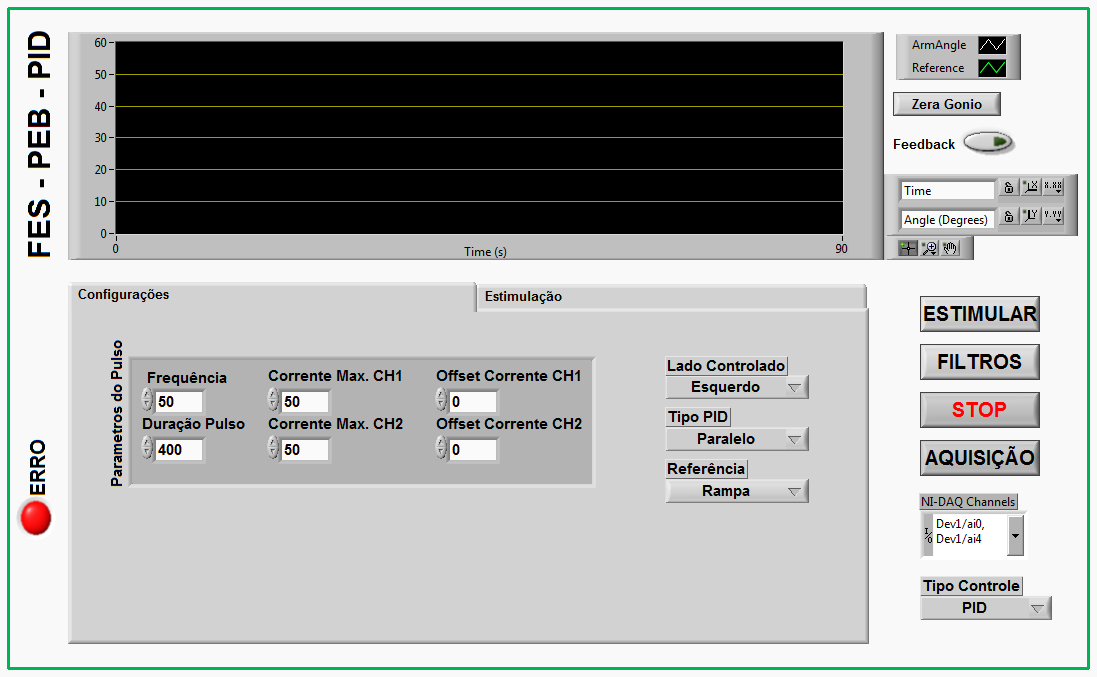
\includegraphics[width=0.8\textwidth]{interface_labview}
	\caption{Tela principal da interface de operação do \textit{software}. Feito em LabVIEW 8.5.}
	\label{fig:interface_labview}
\end{figure}

\paragraph{}A interface com o usuário, explicitada na \ref{fig:interface_labview} possui várias características importantes, um gráfico de exibição em tempo real do ângulo de referência e o do paciente, uma aba de configuração aonde são modificados os parâmetros do pulso, e qual lado está sendo controlado, além de qual estrutura do PID será utilizada, e permite a escolha da referência tanto em rampa quanto contra lateral \ref{label}.

\paragraph{}Os botões na lateral direita fazem o controle de aquisição de dados em tempo real, início da eletroestimulação, e aplicação de filtros para suavizar a referência utilizada \ref{label}. Além de dar a opção de escolher qual dispositivo de aquisição de dados usar, e qual algoritmo de controle a ser implementado.

\subsubsection{\textit{Feedback} Visual}

\begin{figure}[H]
	\centering
	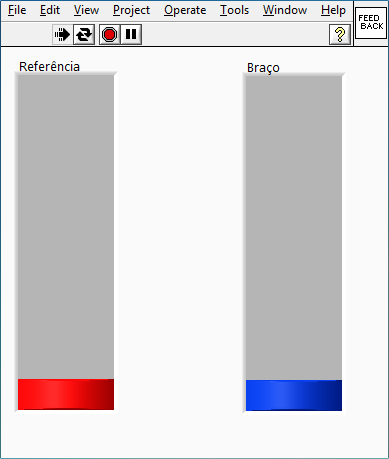
\includegraphics[width=0.8\textwidth]{feedback_visual}
	\caption{Informação visual do ângulo realizado (azul) e a referência (vermelho) em tempo real, com formato de barras crescentes.}
	\label{fig:feedback_visual}
\end{figure}

\paragraph{}O botão de \textit{Feedback} abre a janela de realimentação visual (\ref{fig:feedback_visual}) para os testes com pacientes, aonde a barra azul representa o ângulo realizado em tempo real pelo paciente, e a barra azul a referência.

\section{Testes}
\paragraph{}Para determinar a eficácia do algoritmo, testes com voluntários saudáveis e pacientes acometidos de AVC foram realizados, com isto, um protocolo de testes foi determinado e medidas estatísticas foram efetuadas com o intuito de quantizar esta eficácia.

\paragraph{}Para a realização destes, a pessoa deve ser posicionada no aparato mostrado na \ref{fig:aparatops}, e o ângulo a ser medido no teste é o ângulo $y$ em relação à mesa, exemplificado abaixo.

\begin{figure}[H]
	\centering
	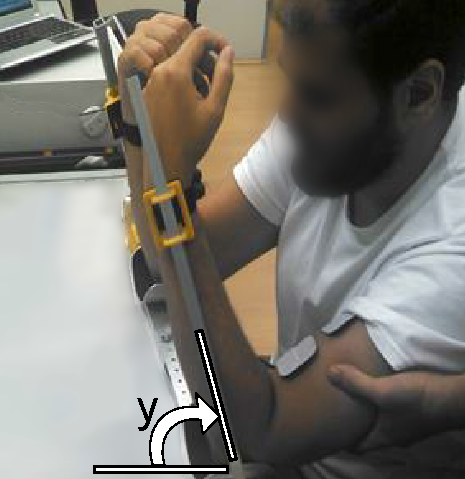
\includegraphics[width=0.6\textwidth]{fig4_new.pdf}
	\caption{Voluntário posicionado no aparelho para a realização dos testes.}
	\label{fig:thiago_anguloy}
\end{figure}


\subsection{Protocolo}
\paragraph{}O protocolo desenvolvido para os testes define o tipo de movimento que o voluntário ou paciente deverá fazer, quais músculos serão estimulados, quais parâmetros de estimulação serão usados e qual é o perfil do voluntário ou paciente passível de realizar o teste.

\paragraph{}O movimento a ser realizado consiste em uma rampa de flexão, um platô de flexão em $45\circ$, depois uma descida em rampa de extensão e finalmente um platô de extensão à $0\circ$.

\begin{figure}[H]
	\centering
	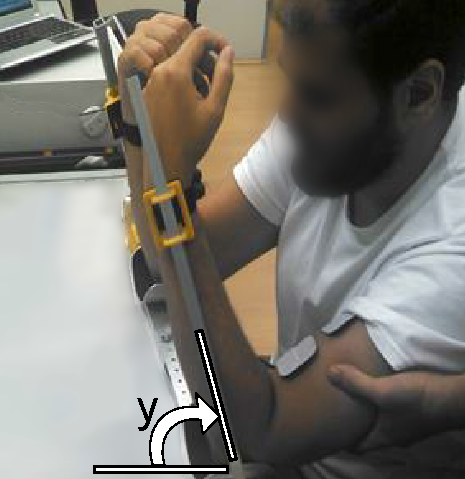
\includegraphics[width=0.5\textwidth]{fig4_new.pdf}
	\caption{Movimento a ser realizado.}
	\label{fig:protocol_mov}
\end{figure}

\paragraph{}Os músculos a serem estimulados serão exclusivamente o bíceps e o tríceps, apenas estimulação de membro superior. Isto foi determinado pois diminui razoavelmente o custo, tendo em vista que os eletrodos para estimulação de membros inferiores são bem maiores e caros.

\paragraph{}Para recrutar os voluntários e pacientes com AVC, foi feita uma triagem dos requerimentos necessários, resumidos abaixo:

\begin{itemize}
	\item Voluntários saudáveis:
	\begin{itemize}
		\item Homens e mulheres de pelo menos 20 anos
		\item 
	\end{itemize}
	\item Pacientes com AVC:
	\begin{itemize}
		\item Possuir um grau de espasticidade mínimo 0 e máximo 3 na escala de Ashworth (\ref{tab:ashworth})
		\item Ser capaz de passar no Mini Mental Test (JOAO!!!)
		\item Mínima capacidade cognitiva (JOAO!!!)
		\item Não ter aplicado BOTOX, ou aplicado à muito tempo
		\item Possuir, em estado de repouso, a capacidade de estender o braço completamente para se posicionar no goniômetro
	\end{itemize}
\end{itemize}

\paragraph{}Antes do início da coleta de dados, é necessário encontrar o ponto motor do músculo. Para fazer isto, foi determinado um procedimento que consiste em estimular o músculo utilizando um eletrodo caneta de $1 cm^{2}$ aumentando gradativamente a amplitude do pulso de estimulação com $1Hz$ de frequência e $400\mu s$ de largura, até que seja observada contração muscular. Após encontrar o ponto aonde a contração seja máxima (mantendo agora a amplitude do pulso fixa), o eletrodo deve ficar posicionado em cima deste.

\paragraph{}Após localizar o ponto motor, um procedimento para determinar a quantidade mínima e máxima de estimulação deve ser feito, este consiste em estimular (agora com os eletrodos fixos) um músculo de cada vez com amplitudes cada vez maiores, usando um pulso agora de $50Hz$ e $400\mu s$. A amplitude que gera a menor contração perceptível deve ser tomada como limite inferior, e a que causa desconforto deve ser tomada como limite superior. Desta forma, podemos realizar os testes com maior facilidade, diminuindo o efeito de zona morta do músculo e evitando desconforto do paciente.

\paragraph{}Depois de todas estas rotinas, o voluntário já poderá realizar o teste de movimento. No contexto de voluntários saudáveis, é necessário que o mesmo se mantenha o mais relaxado possível, com o intuito de não interferir na ação do controlador. Ele também não poderá ter nenhuma ajuda visual ou conhecimento prévio do movimento a ser realizado.

\paragraph{}No contexto de pacientes acometidos por AVC, é necessário que ele atue com o controlador, tendo total conhecimento do movimento a ser realizado, e a ajuda de um estímulo visual em formato de barras (\ref{fig:feedback_visual}), deverá ser instruido ao paciente que ele tente igualar o nível delas.
